% Chapter 3

\chapter{Related Work} % Main chapter title

\label{Chapter3} % For referencing the chapter elsewhere, use \ref{Chapter2} 

%----------------------------------------------------------------------------------------

% Define some commands to keep the formatting separated from the content 
\newcommand{\keyword}[1]{\textbf{#1}}
\newcommand{\tabhead}[1]{\textbf{#1}}
\newcommand{\code}[1]{\texttt{#1}}
\newcommand{\file}[1]{\texttt{\bfseries#1}}
\newcommand{\option}[1]{\texttt{\itshape#1}}

%----------------------------------------------------------------------------------------
\section{The origins: SELF Debugging}\label{SELF}
%SELF needs aggressive optimizations to have reasonable performance. 
%But that prevents from debugging
%Hence OSR enables selective deoptimization at runtime, which provides source level information 
%That makes some optimizations not available since they are hard to undo (e.g. tail %recursion elimination)
%Scope descriptors enable mapping between optimized and unoptimized, enables to keep track %of the position in the virtual call tree etc. (will be detailed). 
%Interrupt points (where, why, how)
%Function invalidation
SELF is a pure object-oriented programming language.
It relies on a pure message-based model of computation that, while enabling high expressiveness and rapid prototyping, impedes the languages performances\cite{chambers1991making, holzle1991optimizing}.
As a result, the language's implementation depends on a set of aggressive optimizations to achieve good performances\cite{chambers1992design, holzle1992debugging}.
SELF provides an interactive environment, based on interpreter semantics at compiled-code speed performances.\\

Providing source level code interactive debugging is hard in the presence of optimizations.
Single stepping or obtaining values for certain source level variables might not be possible.
For a language such as SELF, that heavily relies on aggressive optimizations, implementing a source code level debugger requires new techniques.\\

In \citetitle{holzle1992debugging}\cite{holzle1992debugging}, the authors came up with a new mechanism that enables to dynamically de-optimize code at specific interrupt points in order to provide source code level debugging while preserving expected behaviour.\\

\citean{holzle1992debugging} present the main challenges encountered to provide debugging behaviours, due to the optimizations performed by the SELF compiler. 
Displaying the stack according to a source-level view is impeded by optimizations such as inlining, register allocation and copy propagation.
For example, when a function is inlined at a call site, only a single activation frame is visible, while the source level code expects to see two of them.
Figure \ref{stackframes}, taken from \cite{holzle1992debugging}, provides another example of activations discordances between physical and source-level stacks.
In this figure, the source-level stack contains activations that were inlined by the compiler. For example, the activation B is inlined into A', and hence disappears from the physical stack.\\
\begin{figure}[h]
\centering
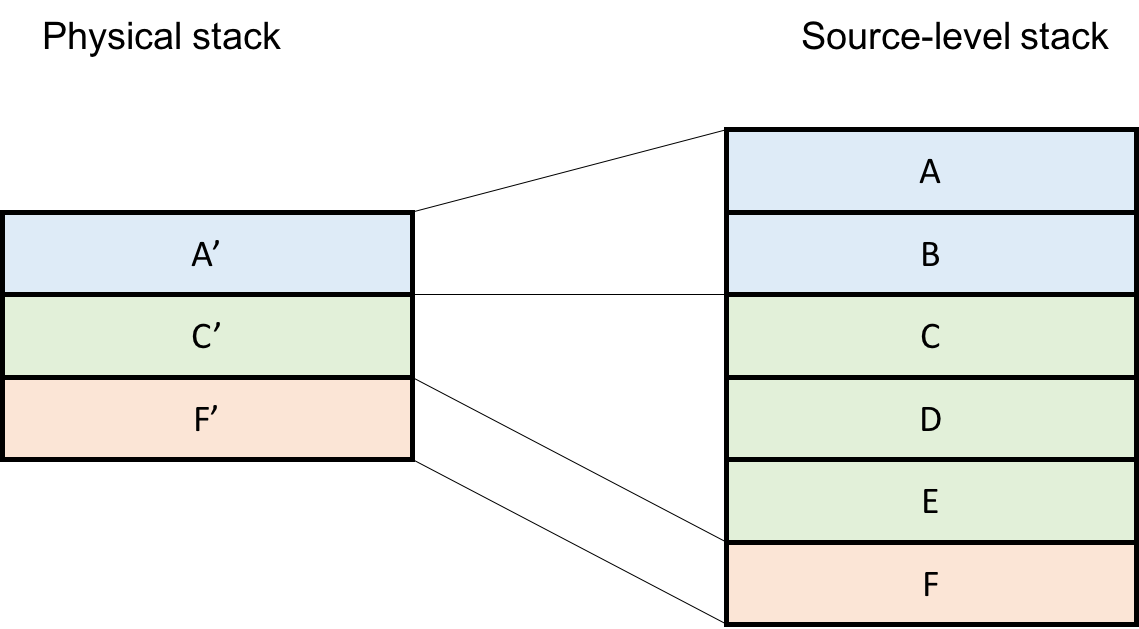
\includegraphics[scale=0.5]{Figures/Figure1}
\decoRule
\caption[physical vs. source-level stacks]{Displaying the stack, figure from \cite{holzle1992debugging}.}
\label{stackframes}
\end{figure}

Single-stepping is another important feature for a debugger. 
It requires to identify and execute the next machine instruction that corresponds to the source operation.
\citean{holzle1992debugging} highlight the impact of code motion and instruction scheduling on the machine instruction layout. 
Such optimizations re-order, merge, intersperse and sometimes delete source-level operations, therefore preventing a straight forward implementation of source-level single-stepping for the debugger.\\

Compiler optimizations prevent dynamic changes from being performed in the debugger.
\citean{holzle1992debugging} identify two separate issues: changing variable values, and modifying procedures (i.e., functions).
To illustrate the first case, the paper\cite{holzle1992debugging} relies on an example where a variable is assigned the sum of two other variables.
The compiler identifies the two variables as being constants and replaces the addition by a direct constant assignment.
A debugger that allows to change variable values at run time would then yield a non correct behaviour if the user modifies one of the two variables. 
This problem does not arise in the case of unoptimized code since the addition is still present. 
For procedures, \citean{holzle1992debugging} provide an example where a function has been inlined by the compiler, but redefined by the user in the debugger.\\

The paper\cite{holzle1992debugging} distinguishes two possible states for compiled code: \textit{optimized}, which can be suspended at widely-spaced interrupt points, from which we can reconstruct source-level state, and \textit{unoptimized}, that can be suspended at any source-level operation and is not subjected to any of the above debugging restrictions.\\

In order to deoptimize code on demand, SELF debugger needs to recover the unoptimized state that corresponds to the current optimized one. 
To do so, it relies on a special data structure, called a \textit{scope descriptor}. 
The scope descriptors are generated during compilation for each source-level scope. 
This data structure holds the scope place in the virtual call tree of the physical stack frame and records locations and values of its argument and local variables. 
It further holds locations or values of its subexpressions.
Along with the scope descriptor, the compiler generates a mapping between virtual (i.e, scope descriptor and source position within the scope) and physical program counters (PC).
Figure \ref{Holzle2} is taken from\cite{holzle1992debugging} and displays a method suspended at two different points. 
At time t1, the stack trace from the debugger displays frame B, hiding the fact that B was inlined inside of A.
At time t2, D is called by C which is called by A, hence, the debugger displays 3 virtual stack frames instead of only one physical frame.\\

\begin{figure}[h]
\centering
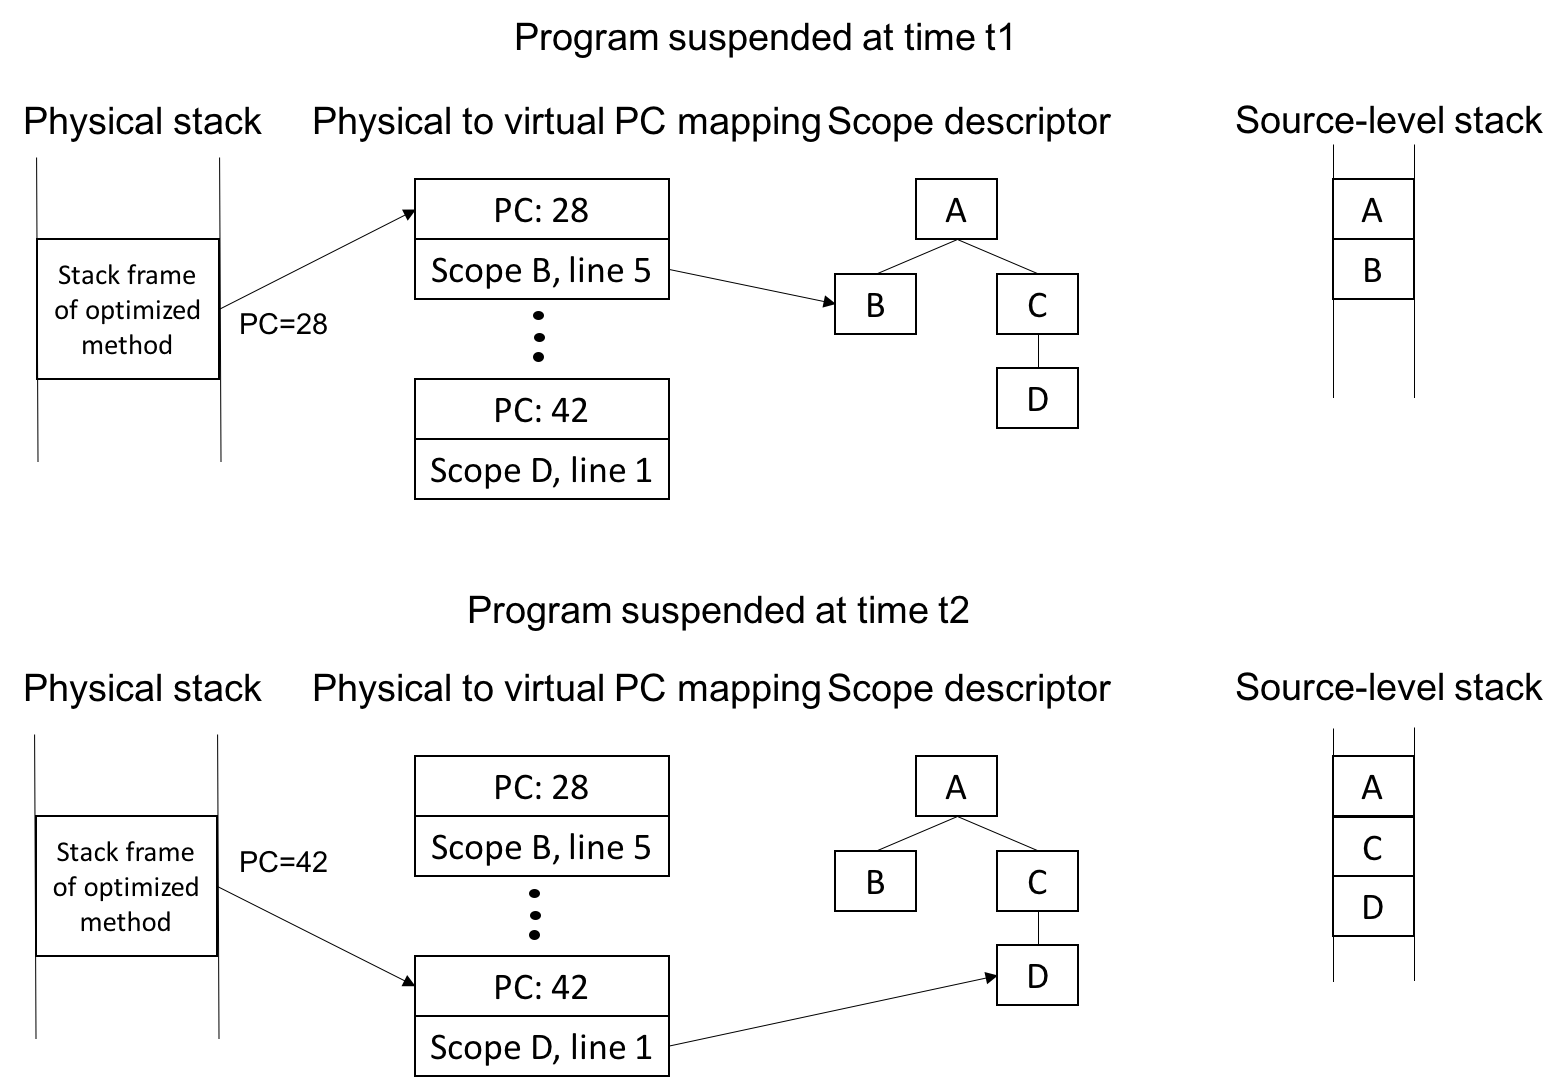
\includegraphics[scale=0.5]{Figures/Figure2}
\decoRule
\caption[Recovering the source-level state]{Recovering the source-level state (from CITE).}
\label{Holzle2}
\end{figure}


The de-optimization process follows 5 steps described in \cite{holzle1992debugging} and summed up here:
\begin{enumerate}
    \item Save the physical stack frame and remove it from the run time stack.
    \item Determine the virtual activations in the physical one, the local variables and the virtual PC.
    \item Generate completely unoptimized compiled methods and physical activations for each virtual one.
    \item Find the unique new physical PC for each virtual activation and initialise (e.g., return addresses and frame pointers) the physical activations created in the previous step.
    \item Propagate the values for all elements from the optimized to the unoptimized activations.
\end{enumerate}

\citean{holzle1992debugging} also describe \textit{lazy deoptimization}, a technique to deoptimize a stack frame that is not at the current top of the execution stack. 
Lazy deoptimization defers the deoptimization transformation until control is about to return into the frame, hence enabling deoptimization for any frame located on the stack.\\

Deoptimization at any instruction boundary is hard. 
It requires to be able to recover the state at every single point of the program.
The SELF debugger relies on a weaker, relaxed restriction by enabling deoptimization only at certain points called \textit{interrupt points}. 
At an interrupt point, the program state is guaranteed to be consistent. 
The paper\cite{holzle1992debugging} defines two kinds of interrupt points: method prologues, and backward branches (i.e., end of loop bodies).
It estimates the length of the longest code sequence that cannot be interrupted to be a few dozen of instruction, i.e., the average length of a code sequence that does not contain neither a call nor a loop end.
Interrupt points are also inserted at all possible run time errors to allow better debugging of synchronous events such as arithmetic overflow. 
The generated debugging information are needed only at interrupt points, which reduces the space used to support basic debugger operations (as opposed to allowing interrupts at any instruction boundary).\\

Providing a debugger for SELF limits the set of optimizations that the compiler can support, and decreases the performances of the program when the execution is resumed. 
Tail recursion elimination saves stack space by replacing a function call with a goto instruction, while fixing the content of registers.
SELF debugger is unable to reconstruct the stack frames eliminated by this optimization and hence, it is not implemented in the SELF compiler.
More generally, tail call elimination is one important limitation for the SELF debugger.

The debugger slows down the execution when the user decides to resume. 
The execution should proceed at full speed, but some stack frames might have been unoptimized, hence implying that a few frames might run slowly right after resuming execution.\\

\section{OSR \& VMs}
Virtual machines are privileged environments in which on-stack replacement can be used to its full power.
As seen in \ref{WhyOSRInteresting}, OSR is as useful as the compiler's profiler is efficient.
A virtual machine (VM) has control over the resources allocation, enables to control the code that is generated by the compiler, maintains important run time data, and state information about the program being executed.
Furthermore, modern virtual machines already provide adaptative strategies to recompile hot functions\cite{arnold2000adaptive, paleczny2001java, holzle1994third, suganuma2001dynamic}, and dispatch calls to the new compiled versions.
OSR enables this transition to happen when the function is executing, rather than during a future call.\\

This section presents several examples of VMs that support on-stack replacement. 
The section is divided into two parts: we first presents several solutions that provide OSR for various virtual machines, then we briefly introduce LLVM, a VM presenting an interesting framework in which we believe on-stack replacement mechanism should fit.\\ 

\subsection{Java HotSpot}\label{HotSpot}

The Java HotSpot Performance Engine is a Java virtual machine developed and maintained by Oracle.
The Java HotSpot VM provides features such as a class loader, a bytecode interpreter, Client and Server virtual machines, several garbage collectors, just-in-time compilation and adaptive optimizations.\\

The Java HotSpot Server Compiler\cite{paleczny2001java} supports on-stack replacement of interpreter frames with compiled-code frames, and deoptimization from compiled-code back to the interpreter.
It relies on adaptative optimizations, that focus on performance critical methods\cite{paleczny2001java, holzle1994third}.
The Java HotSpot Server compiler identifies such methods by using method-entry and backward-branch counters, along with other heuristics related to the method's caller.
Thanks to these counters, the run time system is able to identify frequently executed or long running methods and compile them to improve their run time performance.
It can further decide to compile one or several of the methods callers.
This is called an \textit{upward traversal} and enables to speed the path that leads to a hot method's invocation.  
On-stack replacement is used when the backward-branch counter exceeds the \textit{OnStackReplacementThreshold} value.
The continuation function is compiled with an \textit{additional} entry point at the target of the backward-branch.
A continuation function is therefore able to serve OSR transitions as well as future method invocations.
The run time system transfers the execution from the interpreter to this newly compiled code.\\

In HotSpot, deoptimization might be triggered by two different events: the compilation of a reference to an uninitialised class, and a class loading that invalidates some previous compilation optimization.
Class initialization and class loading are performed by the interpreter. 
Whenever a reference to an uninitialized class is compiled, HotSpot generates an uncommon trap, i.e., a trampoline back to interpreted mode. 
The optimized code is  marked as being unusable, and any thread entering the method are interpreted until the recompilation of the method is achieved properly. 
The second form of deoptimization happens when a class loading invalidates some optimization performed while generating compiled code (e.g., inlining of methods).
A thread that is executing in the invalidated method is "rolled forward"\cite{paleczny2001java} to a safepoint.
When the safepoint is reached, their native frame is extracted and converted into an interpreter frame.
The thread then continues its execution in the interpreter. 
For consistency, the class load that invalidated the compiled method becomes visible to the thread only when it reaches its safepoint.\\

The deoptimization process requires the Java HotSpot to be able to generate an interpreter JVM state at different points of the program.
In order to do so, the Java HotSpot Server records the "exact JVM state"\cite{paleczny2001java} at each safepoint and procedure call.
This implies that the entire JVM state is considered live at the safepoint, which in turns, might extend the live range of some values.
During code emission, the compiler emits a table that maps the JVM state to the resting place of the generated optimized code's JVM state information.\\

\subsection{Jikes RVM}

The Jikes Research Virtual Machine (RVM)\cite{JikesRVMURL} is an open source, self hosted, i.e., it is entirely implemented in Java, virtual machine for Java programs.
One specificity of the Jikes RVM is that it exhibits a \textit{compile-only} approach, i.e., the system compiles all bytecode to native code before execution.
The RVM provides two compilers: a \textit{baseline} compiler, which generates poor quality code quickly, and an \textit{optimizing} compiler. 
The optimizing compiler provides a full suite of optimizations, categorized into three different levels.
The RVM provides advanced state-of-the-art features such as dynamic compilation, adaptive optimizations, garbage collection, thread scheduling and synchronization\cite{JikesRVMURL}.\\

Jikes RVM is an extensible framework in which on-stack replacement techniques have been implemented in two steps, i.e., a first implementation\cite{fink2003design}, and then an extend version of OSR\cite{soman2006efficient}.
%The first
\citean{fink2003design} implemented OSR support in Jikes RVM. 
Their implementation relies on JVM scope descriptor, associated to method activation frames.
A scope descriptor contains the thread running the activation, the bytecode index that corresponds to the program counter, values of all local and stack locations, and a reference to the activation's stack frame.
The OSR transition is divided into three steps: 
\begin{enumerate}
    \item Extract the compiler-independent state from a suspended thread. 
    \item Generate the new code for the suspended activation.
    \item Transfer the execution in the suspended thread to a new compiled code.
\end{enumerate}
\citean{fink2003design} generate the target function by compiling a specialized version of the method for each activation that is replaced, as well as a new version for future invocations.
In other words, instead of allowing multiple entry points per function \cite{lameed2013modular, paleczny2001java}, this JikesRVM OSR implementation generates a specialized version of the target function that has only one entry point, corresponding to the instruction from which the OSR transition was triggered.
Each such method contains a special \textit{prologue}, responsible for saving values into locals and loading values on the stack.
OSR transitions can be taken at special points, called \textit{OSR points}, introduced by the optimizing compiler and that correspond to points where the running activation may be interrupted.
The implementation makes a distinction between unconditional and conditional OSR points.
An OSR point is implemented as a call that takes all live variables as arguments. 
This constraints some optimizations such as dead code elimination, load elimination, store elimination and code motion by extending the liveness scope of some variables.
An OSR point transfers control to an exit block, i.e., it can be viewed as a non-return call.\\

\citean{soman2006efficient} proposed a general-purpose OSR mechanism, for the Jikes RVM, that presents less restrictions for compiler optimizations than the previous approach, while decoupling the OSR implementation from the optimization process.
They extend the previous OSR implementation\cite{fink2003design} to enable OSR transition at, and across points at which the execution can be suspended.
In order to do so, they rely on a special data structure called a \textit{variable map}(VARMAP).
A VARMAP is associated with each method, and consists in a list of thread-switching points and their live variables.
When the compiler performs optimizations, the VARMAP is automatically updated accordingly.
Once the compilation completes, the VARMAP is encoded into a compressed map that contains an entry for each OSR point present in the method.
The VARMAP is decoupled from the compiled code, i.e., it does not influence the liveness of local variables.
\citean{soman2006efficient} also propose an alternative lazy triggering of on-stack replacement.
Lazy triggering consists in taking an OSR transition due to events in the environment, i.e., events triggered by the runtime. 
Whenever the runtime deems an assumption invalide, it invokes a helper function called \textit{OSR helper} that either patches the code of the executing methods to call the OSR process, or it modifies return addresses of the callees of the method to point to the OSR helper.
When a callee returns, the OSR helper creates a new stack frame with the state extracted from the specialized method's stack and saves all of the specialized method registers into its stack frame. 
The return address of the OSR helper points to the current instruction in the specialized code, which is then used during OSR to identify the location to resume the execution in the new version of the method.
Lazy triggering improves the code efficiency by avoiding the extra cost of guards evaluations.\\

\subsection{WebKit VM}\label{webkit}

WebKit\cite{WebKitURL} is an open source web browser engine used to improve JavaScript performances.
It exhibits a Four-Tier VM architecture. 
The WebKit run-time compilation flow is described by Figure \ref{FTL}.\\
\begin{figure}[h]
\centering
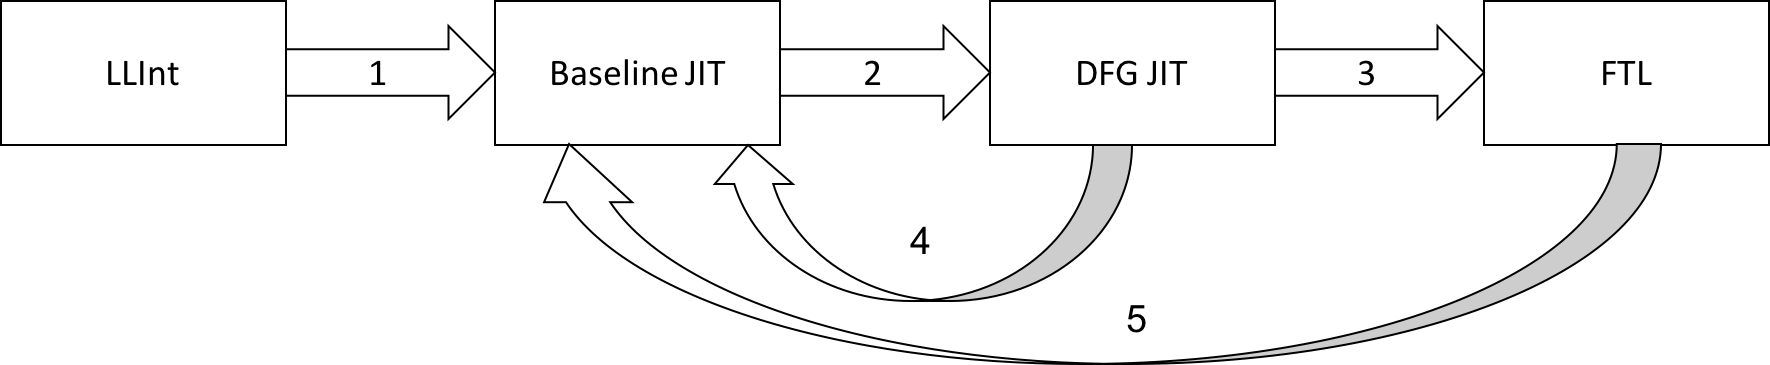
\includegraphics[scale=0.5]{Figures/FTL}
\decoRule
\caption[The WebKit FTL]{The WebKit Four-tier optimization flow.}
\label{FTL}
\end{figure}
 
Forward arrows represent \textit{OSR entries}, i.e., a transformation that yields a more optimized version of the code at run time.
Backward arrows correspond to \textit{OSR exits}, i.e., a transformation that yields a less optimized version of the code at run time.
The low level interpreter (LLInt) is used for low latency start up.
The baseline JIT generates WebKit bytecode with no optimization enabled.
The transition from the first tier to the second one happens when a statement is executed more than a hundred times or a function is called more than six times.
The data flow graph (DFG) JIT is triggered when a statement executes more than a thousand times or a function is called more than sixty-six times.
The Fourth-Tier LLVM(FTL)\cite{WebKitFTL} relies on LLVM machine code optimizations to generate a fast version of portions of the code.
In order to hide the costs of the translation to LLVM IR and its compilation time, the FTL is triggered only for long running portions of the code that are currently executing.
There are two kinds of transitions in WebKit: the ones contained entirely inside the WebKit framework (i.e., transitions 1,2 \& 4 in Figure \ref{FTL}), and the ones that involve LLVM (i.e., 3 \& 5 in Figure \ref{FTL}).\\

Transitions to and from LLVM are hard. 
There is no control over the stack layout or the optimized code produced by LLVM.
In the case of transition 3, a different LLVM version is generated for each entry point that the framework desires to have inside this function.
In WebKit, such entry points are located at loop headers. 
This choice makes sense with regard to the condition to enter the FTL, i.e., transition 3 is taken for long running portions of code that could be improved thanks to LLVM low level optimizations.
WebKit has to generate a different version of the function for each entry points for two main reasons: LLVM allows only single entry points to functions (going around this limitation would require to modify LLVM IR and implementation), and instrumenting a function with several entry points would impact on the quality and performance of the generated native code by extending the code's length and restricting code motion.\\

Performing transition 3 requires to get the current state of execution and identify the entry point corresponding to the current instruction being executed.
The DFG dumps its state into a scratch buffer.
An LLVM function with the correct entry point is then generated, and instrumented such that its first block loads the content of the scratch buffer and correctly reconstructs the state.
The mapping between the DFG IR nodes and the LLVM IR values is straight forward since both IR's are in SSA.
A special data structure, called a Stackmap, enables to keep the mapping between LLVM values and registers/spill-slots.\\

Transition 5 is harder as it requires to extract the execution state from LLVM.
WebKit has two different mechanisms to enables OSR exits: the exit thunk and the invalidation points.
In the first case, WebKit introduces exit branches at OSR exit points.
The branch is guarded by an OSR exit condition and is a no-return tail call to a special function that takes all the live non-constant and not accounted for bytecode values as inputs.
The second mechanism enables to remove the guard.
Since we assume that the portion of code that is instrumented is executed a lot of times, the cost of testing the condition can have a great impact on the overall execution time.
This mechanism relies on special LLVM intrinsics, namely patchpoints and stackmap shadow bytes.
A patchpoint enables to reserve some extra space in the code, filled with nop sleds. 
When the WebKit framework detects that an exit should be taken, it overwrites the nop sleds with the correct function call to perform the OSR exit.
This breaks the optimized version of the code which cannot be re-used later on and must be collected.
The stackmap shadow bytes improves on this technique by allowing to directly overwrite the code, without having any nop sled generated before hand.\\

WebKit is a project that heavily, and successfully relies on OSR to improve performances.
The web browser engine is used in Apple Web browser Safari and enables a net improvement of performances while proving to be reliable.
Although successful, it does not provide a general and reusable framework for OSR in LLVM that other projects could benefit from.\\

\section{OSR \& LLVM}\label{OSR&VM}
\subsection{What is LLVM?}
%TODO cite the llvm paper?
LLVM\cite{llvmUrl, lattner2004llvm}, formerly called Low-Level Virtual Machine, is a compiler infrastructure that provides a set of reusable libraries.
LLVM provides the middle layers of a compiler system and a large set of optimizations for compile-time, link-time, run-time, and idle-time for arbitrary programming languages.
These optimizations are performed on an intermediate representation (IR) of the code and yield an optimized IR.
The LLVM framework also provides tools to convert and link code into machine dependent assembly code for a specific target platform.
LLVM supports several instruction sets including ARM, MIPS, AMD TeraScale, and x86/x86-64\cite{llvmUrl}.\\

The LLVM intermediary representation is a language-independent set of instructions that also provides a type system.
The LLVM IR is in static single assignment (SSA) form, which requires every variable to be defined before being used, and assigned exactly once. 
SSA enables or improves several compiler optimizations among which constant propagation, value range propagation, sparse conditional constant propagation, dead code elimination, global value numbering, partial redundancy elimination, strength reduction, and register allocation\cite{appel1998ssa}.
The SSA requirement for variables to be assigned only once requires a special mechanism, called a $\phi$-node, when a value depends on which control flow branch was executed before reaching the current variable definition.
Figure \ref{SSA example} provides an example where we have to choose between two possible values for a variable after the merging of two control flow branches.\\

\begin{figure}[h]
\centering
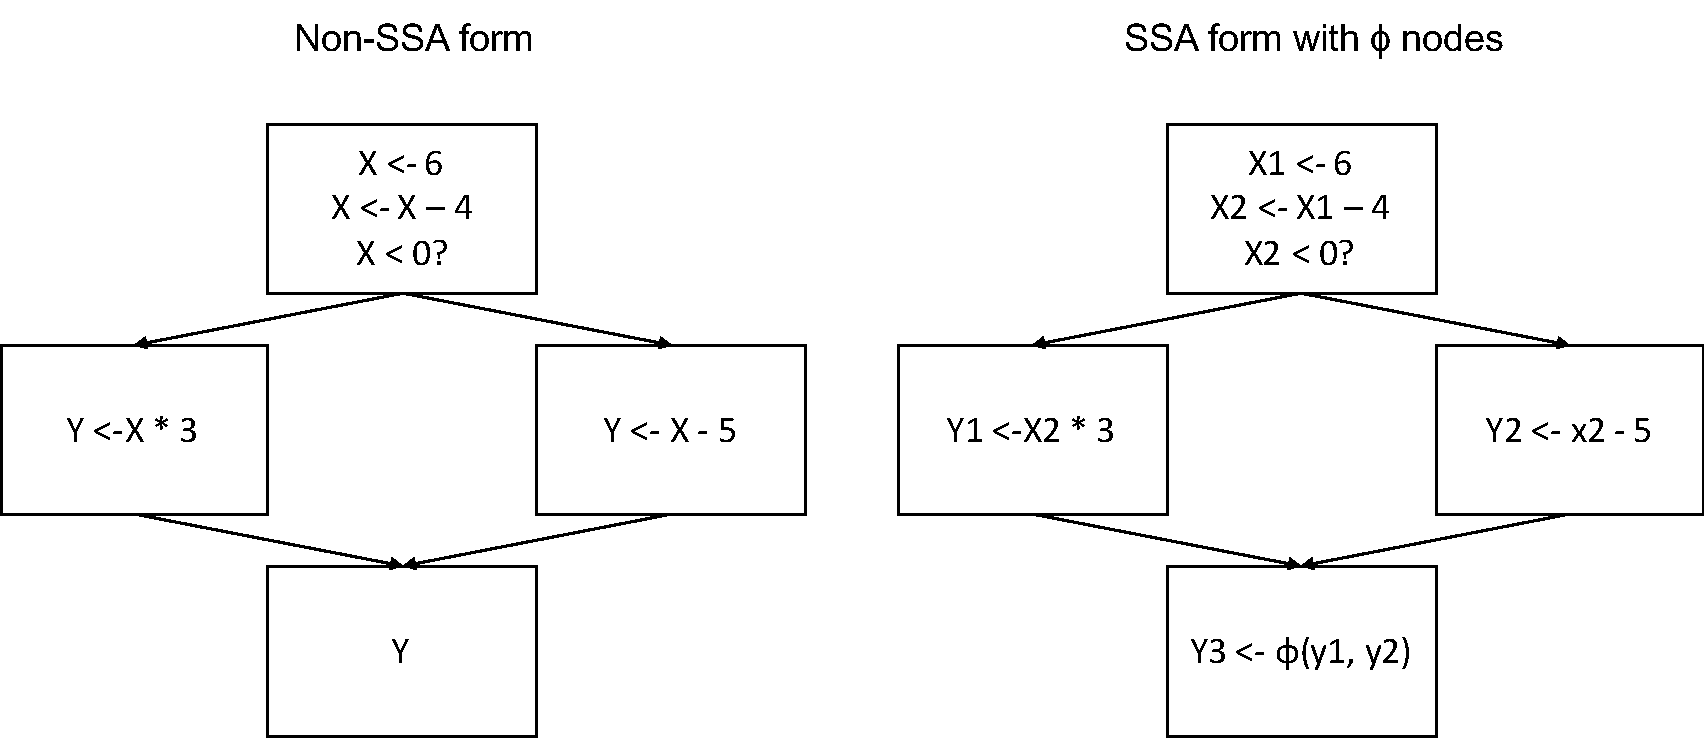
\includegraphics[scale=0.5]{Figures/SSAForm}
\decoRule
\caption[SSA example]{Example of $\phi$-node in SSA form.}
\label{SSA example}
\end{figure}

%TODO exhaustive basic types?
The LLVM IR type system provides basic types (e.g., integers, floats), and five derived types: pointers, arrays, vectors, structures, and functions.
Any type construct can then be represented as a combination of these types.\\

%TODO reformulate/restructure this §
The LLVM framework is a versatile tool that enables to implement many programming languages paradigms.
LLVM-based compilers exist for several mainstream/popular languages such as Java, Python, Objective-C, and Ruby.
Other languages, like Haskell, Scala, Swift, Rust, Ada, and Fortran also have an LLVM compiler implementation.
LLVM basic types enable to support object-oriented languages, such as Java and Python, dynamically typed languages like R, or statically typed like Scala.
LLVM also enables to model functional languages such as Haskell, as well as imperative ones. 
Furthermore, it supports reflection and, thanks to dynamic linking, modular languages (e.g., Haskell).
The tools provided enable static compilation as well as dynamic compilation techniques such as Just-In-Time compilation (JIT).\\

\subsection{Why do we want OSR in LLVM?}

On-stack replacement high-level mechanism is language-independent.
Therefore, implementing OSR as a clean modular addition to LLVM would enable developers to leverage this feature in many programming languages, without requiring them to write a new compiler from scratch.
Furthermore, as explained in \ref{WhyOSRInteresting}, OSR is a useful tool for dynamic and adaptative optimizations.
LLVM already provides implementations for many compiler optimizations\cite{llvmUrl} and tools to allow dynamic recompilation of code.
Developers can therefore focus on language specific challenges, such as efficient profilers and new speculative systems, rather than on the optimizations and OSR implementations.\\

Implementing OSR for LLVM not only serves several languages, but also allows to provide a solution for several target platforms.
As explained previously, LLVM supports several instruction sets corresponding to different architectures.
By implementing OSR in LLVM, we get portability among these platforms for free.\\

\subsection{OSR as an LLVM library: the McOSR implementation}\label{McOSR}
The McOSR OSR support\cite{lameed2013modular} is an attempt at providing an OSR library compatible with the standard LLVM implementation. 
Lameed \& Hendren claim to have come up with a clean modular, and re-usable technique completely defined at the LLVM IR level and compatible with the standard LLVM distribution.
The implementation has been tested in the MvVM/McOSR\cite{chevalier2010optimizing, McVM}, an open source VM and JIT for MATLAB, built on LLVM.
Their implementation answers to five challenges, listed in the paper\cite{lameed2013modular}, and reproduced here:\\ 

\begin{enumerate}
    \item Identifying correct interrupt points and using the current LLVM IR to represent them.
    \item Using the LLVM tools to correctly transform the IR while preserving a correct control flow graph. 
    \item Making a new version of a function available at the same address as the old one.
    \item Providing a clean API for the OSR library, that is compatible with LLVM's inlining capabilities.
    \item Integrating OSR without modifying the LLVM installation.
\end{enumerate}

\citean{lameed2013modular} claim to support optimization and re-optimization, as well as de-optimization by going back to the previous version of the function.
Figure \ref{OSR classification} shows that this feature only allows single-steps to be taken, i.e., the OSR library implemented in\cite{lameed2013modular} does not seem to allow to skip intermediary versions.\\

\begin{figure}[h]
\centering
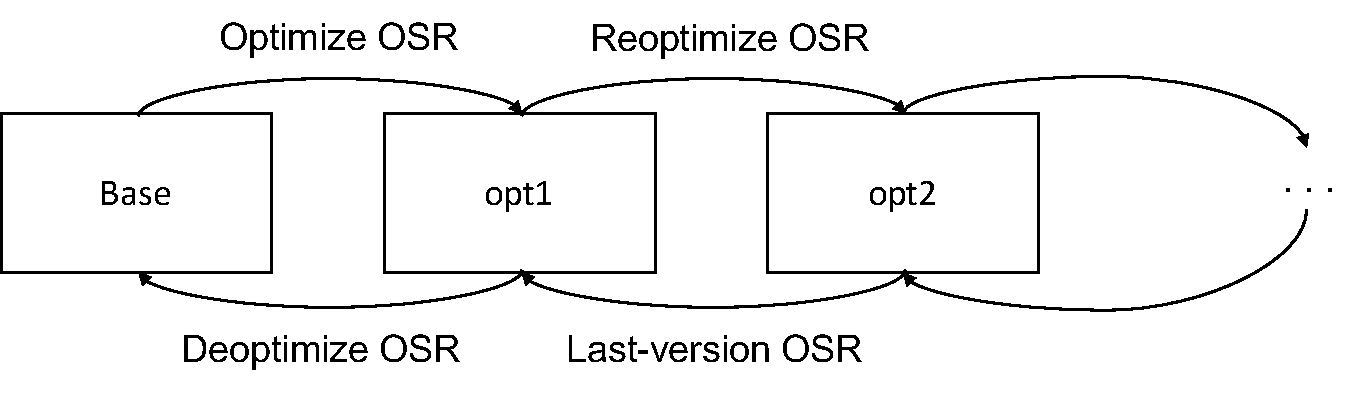
\includegraphics[scale=0.5]{Figures/OSRClassification}
\decoRule
\caption[OSR classification]{OSR classification from\cite{lameed2013modular}.}
\label{OSR classification}
\end{figure}

The McOSR library that provides OSR functionalities fit into the regular JIT infrastructure provided by LLVM as described in Figure \ref{McOSRArchitecture} taken from\cite{lameed2013modular}. 
\begin{figure}[h]
\centering
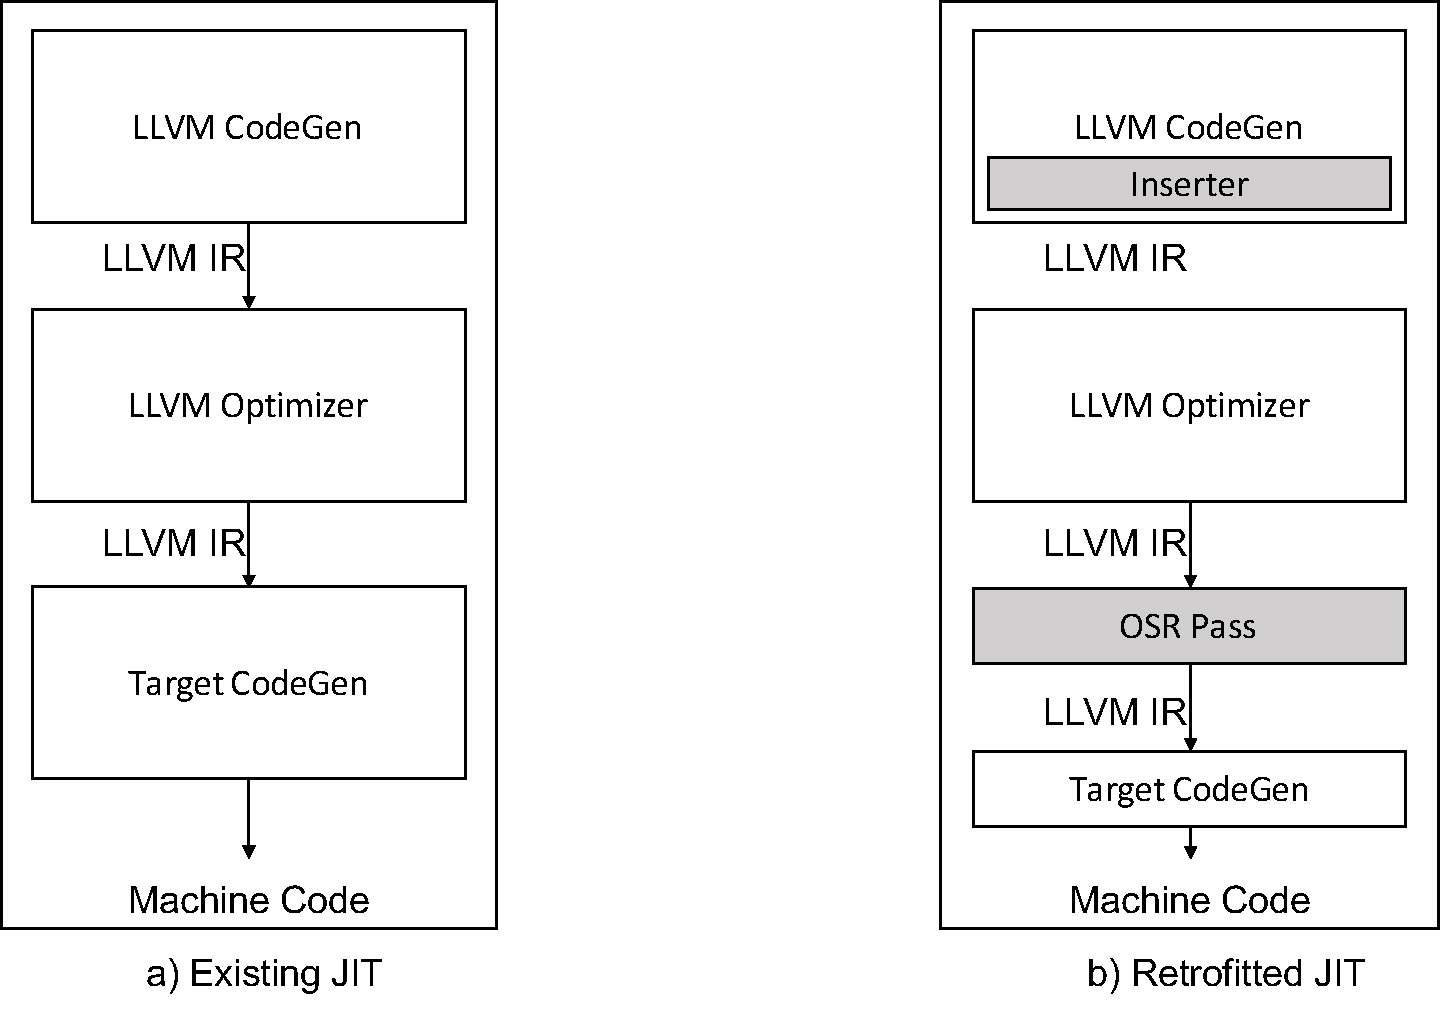
\includegraphics[scale=0.5]{Figures/MCJitArchitecture}
\decoRule
\caption[Retrofitting an existing JIT with OSR support]{Retrofitting an existing JIT with OSR support from CITE}
\label{McOSRArchitecture}
\end{figure}
The left figure is a normal JIT in LLVM. 
The LLVM CodeGen is the front-end of the compiler infrastructure that generates the LLVM IR.
The LLVM Optimizer contains a collection of transformations and optimizations that run on LLVM IR. 
The Target CodeGen outputs the machine code corresponding to the LLVM IR input. 
The McOSR API instruments the LLVM CodeGen to insert OSR points where the OSR transition can be triggered. 
A point is a call to the genOSRSignal function, which takes as arguments a pointer to a code transformer responsible for generating the new version of the function.
The code transformer takes as arguments a pointer to the function that needs to be transformed, and a special OSR label to identify which OSR point triggered the call, if the function contains several ones.
The OSR pass is responsible for instrumenting OSR points with the correct OSR machinery.
The instrumentation saves the live values and creates a descriptor that contains four elements: 
%TODO explain the control version better
\begin{enumerate}
    \item A pointer to the current version of the function. 
    \item A pointer to the control version of the function, i.e., a copy of the old version of the function.
    \item A variable mapping between the original version and the control version.
    \item The set of live variables at the OSR points. 
\end{enumerate}\\

\begin{figure}[h]
\centering
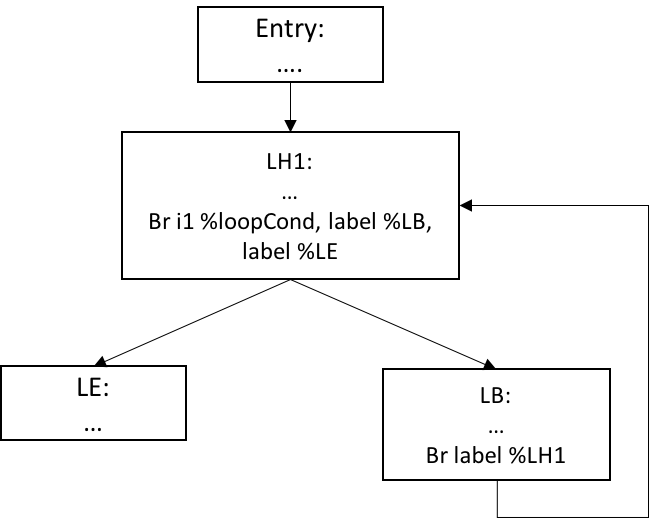
\includegraphics[scale=0.5]{Figures/BaseCFG}
\decoRule
\caption[A CFG of a loop with no OSR point]{A CFG of a loop with no OSR point from\cite{lameed2013modular}.}
\label{BaseCFG}
\end{figure}

\begin{figure}[h]
\centering
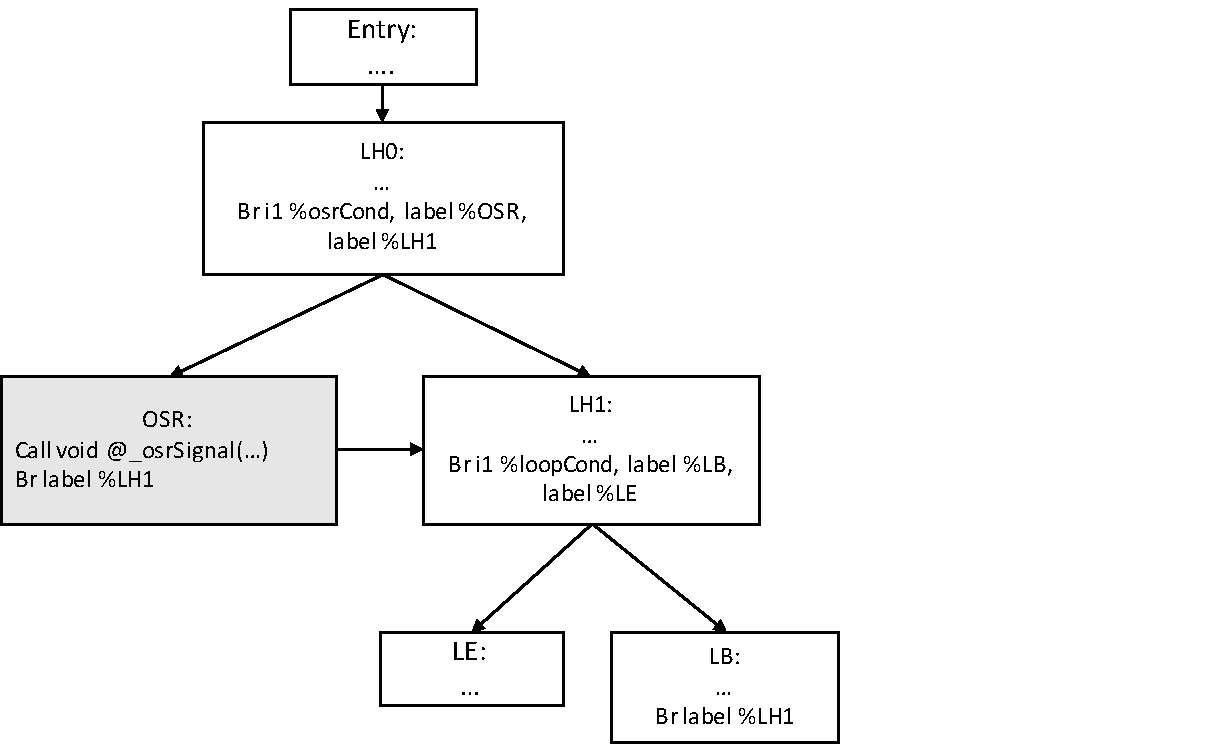
\includegraphics[scale=0.5]{Figures/InsertCFG}
\decoRule
\caption[The CFG of the loop in Figure \ref{BaseCFG}, after inserting an OSR point]{The CFG of the loop in Figure \ref{BaseCFG}, after inserting an OSR point from\cite{lameed2013modular}.}
\label{InsertCFG}
\end{figure}

\begin{figure}[h]
\centering
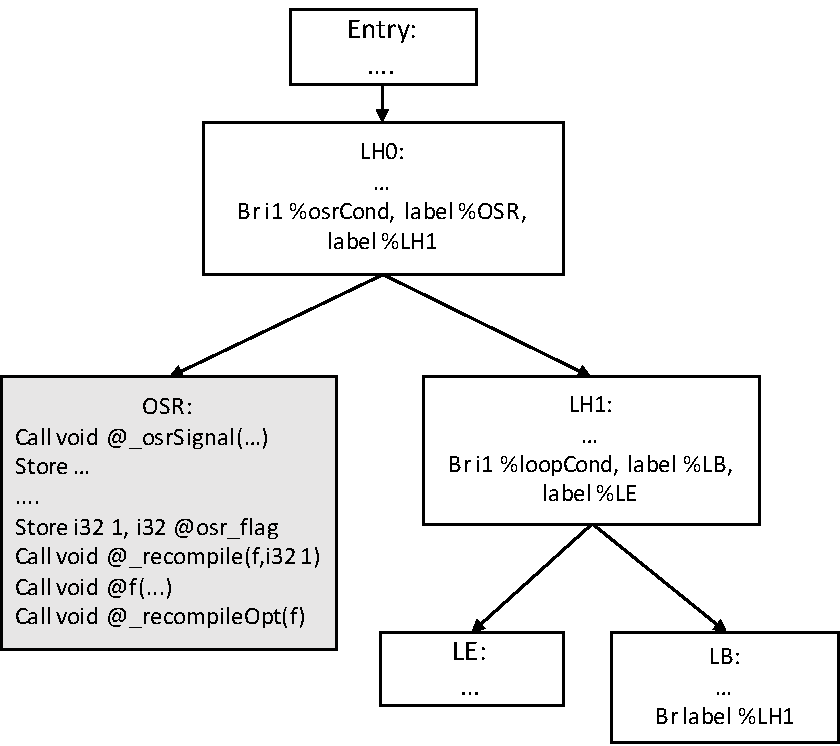
\includegraphics[scale=0.5]{Figures/OSRPassCFG}
\decoRule
\caption[The transformed CFG of the loop in Figure \ref{InsertCFG} after the OSR Pass]{The transformed CFG of the loop in Figure \ref{InsertCFG} after the OSR Pass from\cite{lameed2013modular}.}
\label{OSRPassCFG}
\end{figure}\\

Figures \ref{BaseCFG}, \ref{InsertCFG}, and \ref{OSRPassCFG} give an example of OSR instrumentation at a loop header.
LH1 is the loop header. 
LB is the body of the loop and LE the loop exit. 
Figure \ref{BaseCFG} control flow graph (CFG) is the original CFG. 
Figure \ref{InsertCFG} is the resulting CFG after the Inserter is executed.
Figure \ref{OSRPassCFG}'s CFG corresponds to the result of the OSR pass.
The \textit{recompile} call in the OSR block recompiles \textit{f} using the correct code transformer.
Then \textit{f} calls itself, executing the new version of the function.
This works since the new version lives at the same address as the previous one and is instrumented to jump to the correct instruction, i.e., the one corresponding to the current point at which OSR was triggered.
Figure \ref{FCFG} represents the CFG of \textit{f} before the OSR instrumentation.
Figure \ref{InstFCFG} shows the instrumentation of \textit{f} that enables to jump to the correct instruction in the middle of the function. 
A prolog entry block is inserted at the function header.
This block checks the \textit{OSR flag} to know if an OSR transition is being performed.
If that is the case, it branches to the prolog block that restores the state before resuming the execution at the correct instruction.\\

\begin{figure}[h]
\centering
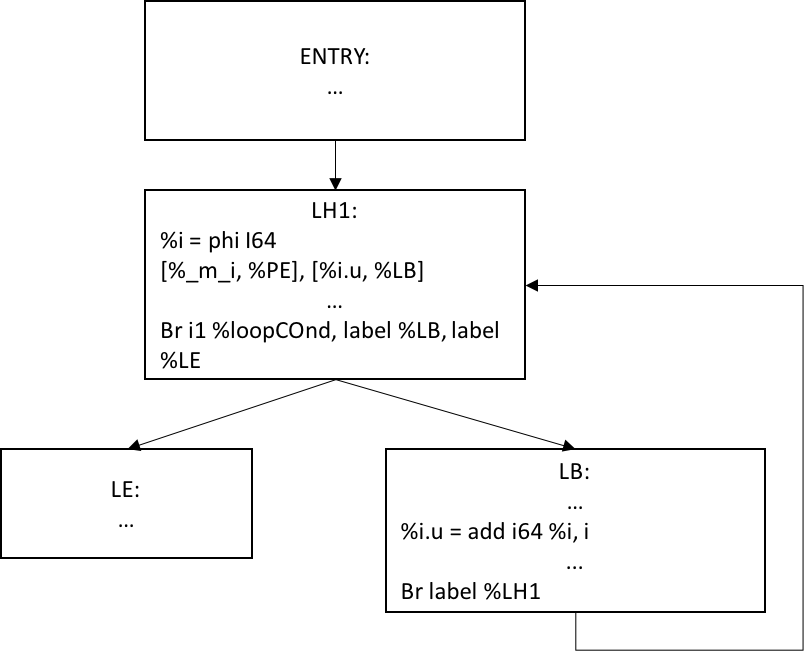
\includegraphics[scale=0.5]{Figures/FCFG}
\decoRule
\caption[A CFG of a running function before inserting the blocks for state recovery]{A CFG of a running function before inserting the blocks for state recovery, from\cite{lameed2013modular}.}
\label{FCFG}
\end{figure}

\begin{figure}[h]
\centering
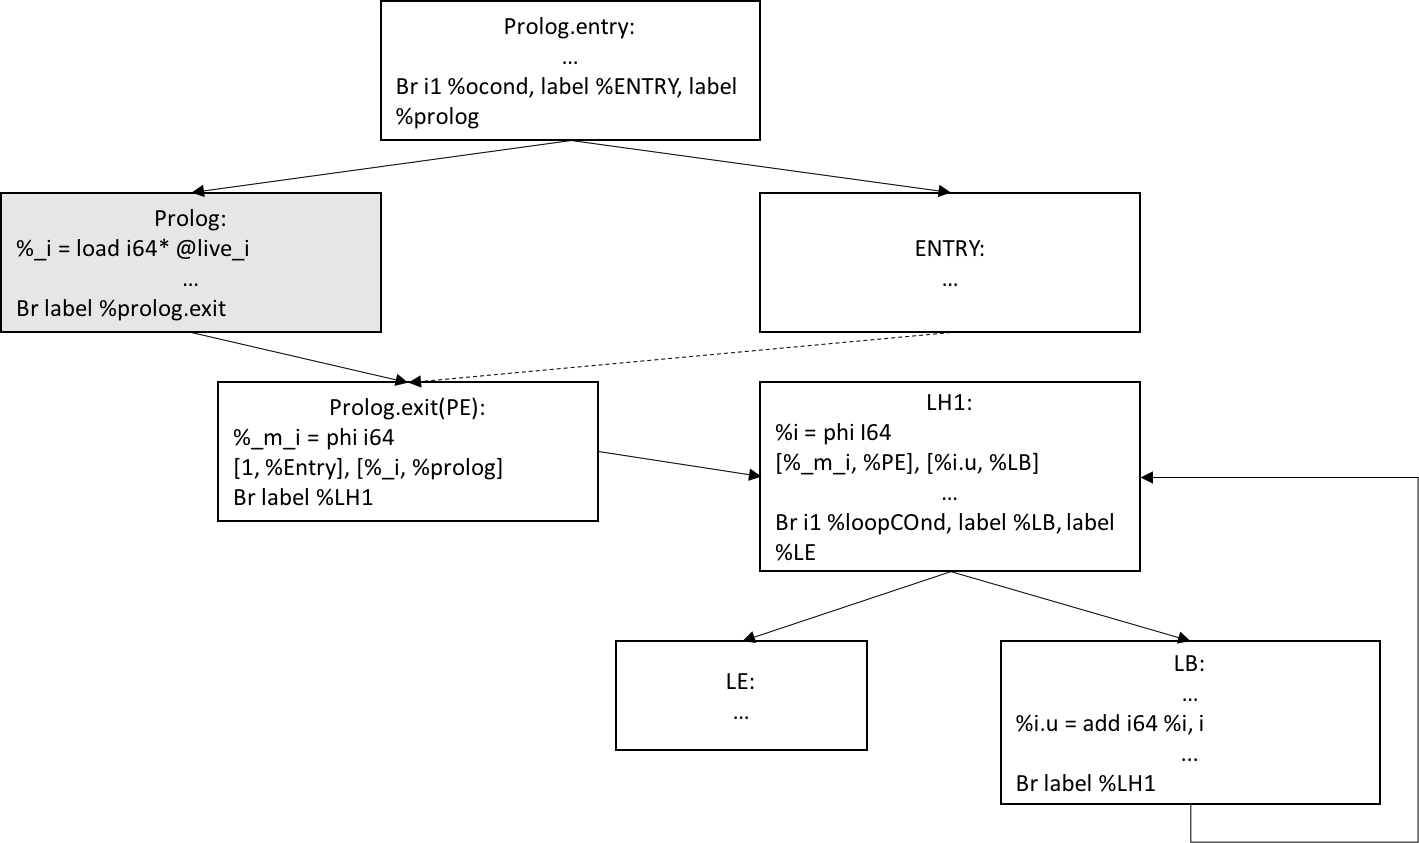
\includegraphics[scale=0.5]{Figures/FOptCFG}
\decoRule
\caption[The CFG of the loop represented in Figure \ref{FCFG} after inserting the state recovery blocks, form\cite{lameed2013modular}.]{The CFG of the loop represented in Figure \ref{FCFG} after inserting the state recovery blocks, form\cite{lameed2013modular}.}
\label{InstFCFG}
\end{figure}\\

%TODO critic of the paper.
The OSR implementation proposed in\cite{lameed2013modular} presents interesting features.
The implementation is done entirely at the LLVM IR, hence making it language-independent.
Furthermore, since the transformation function is provided by the user, any kind of language specific transformation can be used during the OSR.
As a result, McOSR support is a modular, and general purpose OSR library.\\

On the other hand, this library does not allow to have several versions of the same function live at the same time.
This restriction can impede the overall performance of the program by extending the scope in which an assumption on which we base the transformation must hold.
For example, a portion of the code, call it \textit{A}, can trigger an OSR, while portion \textit{B} is such that the assumption on which the optimization is based does not hold.
The choice that the user has is to either optimize for A, and deoptimize for B, or to prevent A from optimizing by enlarging the scope in which the assumption is supposed to hold.
None of these solutions is good if \textit{A} and \textit{B} are executed many times, one after the other.
We will either lose a lot of execution time performing OSR, or keep executing \textit{A} without optimization.\\

In the paper, the deoptimization process is not described. 
It is implied that it relies on the same set of tools provided by the framework as the optimization process, but no example is provided.
As explained in \ref{WhyOSRInteresting}, deoptimization is the most interesting feature of OSR, as it is required to preserve correctness.
Being able to identify where a function should exit is a hard task.
The McOSR library does not provide tools to ease this process and leaves the responsibility to the developer to instrument his functions correctly in order to exit to the correct landing pad.\\

To the best of our knowledge, McOSR library is not currently used in production or any important project.
As mentioned earlier, WebKit is efficiently integrated in Apple Safari's web browser, which provides useful feedback on its performances.
The lack of usage of McOSR library prevents us from collecting performance results and assess its efficiency.
Furthermore, the experimental evaluation in\cite{lameed2013modular} relies on an example that seems artificial for our use of OSR. 
The case study presents a dynamic inliner that decides to inline a function call if the function is less than 20 basic blocks long, or if it is less than 50 basic blocks long and has an interpreter environment associated with its body. 
This requirement for inlining is one that can be checked statically and, hence, seems a little artificial.\\

\subsection{Another LLVM OSR library: OSR Kit}\label{describeOSRKit}
OSR Kit\cite{OSRKit} is a general purpose, target independent, implementation of on-stack replacement for LLVM.
As such, it can be used by any LLVM based compiler.
The main goals of the OSR Kit project are:
\begin{enumerate}
    \item To allow chained OSR transitions, i.e., a continuation function can be instrumented to allow OSR transitions.
    \item To support OSR entries and exits via the same instrumentation.
    \item To allow transitions at arbitrary function locations.
    \item To allow continuation functions to be either generated at run time, or already known at compilation time (i.e., generated on the fly or cached).
    \item To encapsulate and hide the OSR implementation details from the front-end.
    \item To encode OSR transitions entirely at the LLVM IR level.
    \item To limit the intrusiveness of the OSR instrumentation.
    \item To allow the LLVM's compilation pipeline to generate the most efficient native code for an instrumented function. \label{llvmTransformPasses}
\end{enumerate}

The OSR Kit library's main contribution is the implementation of an efficient and flexible OSR transition mechanism.
This transition can be used to implement OSR entries and OSR exits alike.
OSR points are allowed to be inserted at any instruction boundary. 
The OSR library is designed to give the user as much freedom as possible.\\

OSR Kit provides mechanisms for generating the continuation function on the fly or reusing a cached version.
Where other implementations, such as McOSR\cite{lameed2013modular}, made a clear choice between the two techniques, the OSR Kit library decided to enable both of them, hence allowing the user to experiment and select the design that better suits specific use cases.\\

OSR Kit strives for non-instrusive instrumentation of the code in order to have as little impact as possible on the LLVM transformation passes performances.
One of the main advantages of using the LLVM framework is that LLVM transformation passes and optimizations can be automatically added to the compilation pipeline in order to improve the quality of the code generated.
A heavy instrumentation of the LLVM IR might impede on the performances observed for such passes.\\

\subsubsection{Open vs. Resolved OSR}

The \textit{open OSR} scenario corresponds to the case where the continuation function is generated on the fly, when the OSR transition is fired.
Deferring the compilation of the continuation function allows profiled-guided compilation strategies to gather as much information as possible about the current state of the execution, and therefore generate the best possible code.\\

The open OSR scenario is implemented as a call to a stub function, call it $f_{stub}$.
The $f_{stub}$ function is responsible for generating the continuation function, and then transferring the execution to it.
The $f_{stub}$ function receives all the values live at the OSR point as input, and propagates them to the continuation function.
The continuation function is generated by a special \textit{gen} function, that takes as inputs the base function $f$, i.e., the from function, and the OSR point that triggered the transition.\\
%TODO code for the OSR points open. 

Figure REF corresponds to the signature of the OSR Kit function that enables to insert open OSR points.
The \textit{destFunGenerator} is the $f_{stub}$ function and is of type \textit{DestFunGenerator}, described in Figure REF.\\

\begin{figure}[h]
\includecode{Code/DestFunGenerator.c}
\caption{The DestFunGenerator type.}
\label{fig:destfungenerator}
\end{figure}

\begin{figure}[h]
\includecode{Code/OpenOSR.c}
\caption{The insertOpenOSR prototype.}
\label{fig:insertopenosr}
\end{figure}

The open OSR is similar, in theory, to the McOSR implementation\cite{lameed2013modular}.
Both of them rely on a \textit{gen} function to generate the continuation function when the OSR transition is fired.
However, \citean{OSRKit} made the choice to perform these operations, i.e., generating the continuation function and transferring the execution, inside a separated function, rather than instrumenting the from function directly.
This choice was made in order to minimize the code injected inside the from function.
In fact, the instrumentation, even when inserted in a separated branch, might interfere with compiler optimizations.
Examples of such interferences are the increase of register pressure, the alteration of code layout and instruction cache behavior.\\

The \textit{resolved OSR} scenario corresponds to the case where the continuation function is known prior to fire the OSR transition, and the from function has been instrumented to transfer the execution to this specific compiled version.
In the resolved OSR scenario, the transition is expected to be faster than in the open scenario, since there is no compilation to be performed. 
This technique also enables to reuse functions that were compiled previously, e.g., either because several from functions have the same continuation function, or because an OSR point is fired several times during the execution of the program.\\

The resolved OSR is implemented as a call to the continuation function, which takes as inputs all the live variables at the OSR point as inputs.
The continuation function is instrumented to jump at the correct location inside the code to resume the execution. 
Figure \ref{ResolvedOSRFig} illustrates the resolved OSR scenario.\\

\begin{figure}[h]
\centering
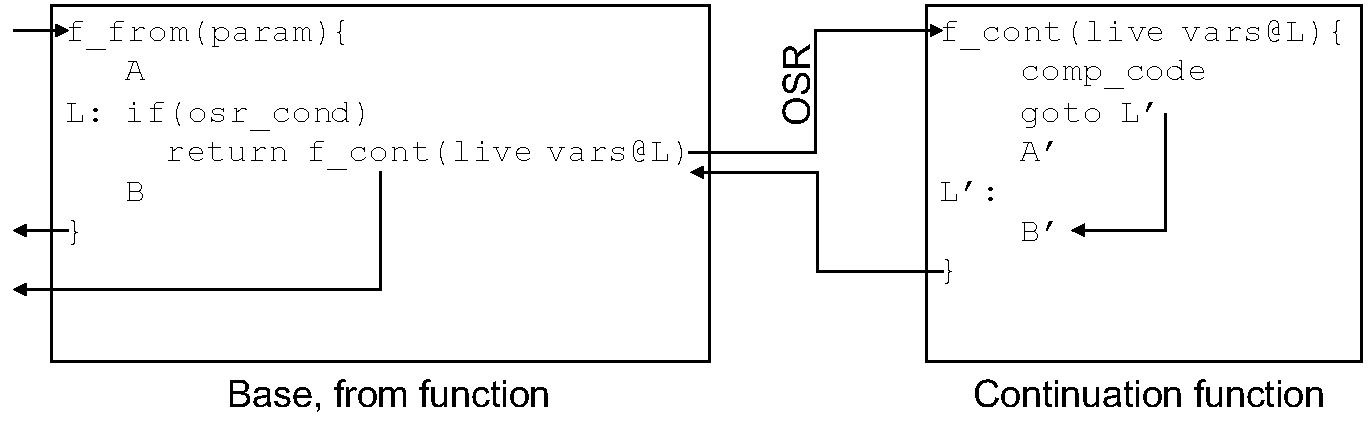
\includegraphics[scale=0.5]{Figures/OSRKitResolvedScenario}
\decoRule
\caption[Resolved OSR Scenario]{Resolved OSR scenario, from\cite{OSRKit}.}
\label{ResolvedOSRFig}
\end{figure}

Figure REF corresponds to the signature of the OSR Kit function that enables to insert resolved OSR.\\

\begin{figure}[h]
\includecode{Code/ResolvedOSR.c}
\caption{The insertResolvedOSR prototype.}
\label{fig:insertresolvedosr}
\end{figure}

\subsubsection{Resolved OSR points and conditions}
In the OSR Kit library\cite{OSRKit}, there is no distinction at the implementation level between OSR exits and entries.
The general mechanism used is the OSR point.
An OSR point corresponds to a labelled LLVM basic-block that contains the call to the continuation function and the return instruction to propagate the result of the call.
OSR points are protected by an OSR condition. 
The OSR Kit library allows an OSR condition to be any vector of LLVM instructions. 
The last instruction is automatically used by the framework as condition for an LLVM branch instruction. 
If the condition succeeds, the OSR transition is fired.
Otherwise, the execution continues in the function.\\

Figures REF and REF provide an example of OSR instrumentation.
In Figure REF, we have the R declaration of two functions, $f$ and $g$, and the simplified LLVM IR generated for $g$ in RJIT.
Figure REF presents the instrumented version of $g$, in which a resolved OSR point has been inserted.
Lines 5 and 6 correspond to the OSR condition.
In this example, the OSR is fired if line 1 does not yield the same function for $f$ as the one that was used by the RJIT compiler when it generated the instrumented function.
If the OSR is fired, the execution jumps to the \textit{OSR\char`_fire} basic block and calls the continuation function, namely \textit{OSRCont}.
The OSR point \textit{OSR\char`_fire} calls the continuation and propagates its return value line 15.
The \textit{OSR\char`_split} block corresponds to the regular continuation of the function $f$ when the OSR is not fired.\\

\begin{figure}[h]
\includecode[asm]{Code/original.llvm}
\caption{Simplified original LLVM IR.}
\end{figure}

\begin{figure}[h]
\includecode[asm]{Code/fromInstrumented.llvm}
\caption{Simplified instrumented LLVM IR.}
\end{figure}

\subsubsection{The continuation function \& StateMap}

The OSR Kit library heavily relies on a special object, called a \textit{StateMap}, to keep a mapping between the from function and the continuation function.
The StateMap enables to register unidirectional and bidirectional mappings between LLVM instructions and function arguments.
The default constructor for a StateMap relies on the LLVM ValueToValueMapTy\cite{VMap}(VMap) to automatically extract the mappings.
A VMap can be filled with such mappings when the LLVM cloning functions are used, i.e., the OSR Kit encourages you to generate the continuation function by cloning either the base or the from function such that a VMap is already available when the framework needs to introduce the instrumentation.
The StateMap also provides an API to register and unregister mappings by directly providing the two instructions.\\

Both deoptimization and optimization rely on the same kind of continuation functions, and on the same instrumentation tools.
A continuation function, in OSR Kit, has a special function signature that takes as inputs all the variables that were live at the instruction at which the OSR transition was fired.
Its return type is the same as the from and the base (unmodified and un-instrumented) functions.
The OSR Kit instrumentation inserts a special basic block, called \textit{OSR ENTRY}, at the beginning of the continuation function.
The OSR ENTRY is responsible for executing the \textit{compensation code} and jumping to the correct block inside the continuation function.
The compensation code is specified by the user as a vector of instructions associated with a source value, when the OSR is inserted in the code.
The continuation instruction, i.e., the instruction to which the OSR ENTRY jumps to is assured by the OSR Kit library to be the first instruction in the destination block.
Everything between the OSR ENTRY and the continuation block becomes dead code.
The dead instructions are automatically eliminated by the LLVM transformation passes.
In any case, their only impact is on the space used up by the program, their presence does not increase the execution time of the continuation function.
It might, however, impact on later optimizations performed on the code.\\

CODE EXAMPLE.\\

\citean{OSRKit} claim that passing live values as arguments to the continuation function is more efficient than loading them from a buffer.
According to \cite{fink2003design}, generating a dedicated function to resume the execution to continue the execution, as opposed to instrument a general function to serve as continuation as well as a regular function, is expected to lead to better results.
In other words, it is supposed to be better to keep the base function to serve regular calls, and trigger OSR transitions whenever we need them, during the execution of the function.
This claim is debatable in the case of deoptimization.
Chapter\ref{Chapter4} expands on the question.\\

\section{A classification summary}
%TODO some kind of sum up and comparison, related to what we had in chapter 2.
This section presents a summary of the various OSR implementations presented in this Chapter.
The summary is presented in Table \ref{tab:Summary} and focuses on the state propagation technique, the types of OSR points supported, the implementation of the transition mechanism, and the target of OSR exits.\\

\clearpage

\begin{landscape}
\begin{table}[h!]
\centering
\begin{tabular}{|p{\dimexpr 0.12\linewidth-2\tabcolsep}|
                 p{\dimexpr 0.12\linewidth-2\tabcolsep}|
                 p{\dimexpr 0.12\linewidth-2\tabcolsep}|
                 p{\dimexpr 0.12\linewidth-2\tabcolsep}|
                 p{\dimexpr 0.12\linewidth-2\tabcolsep}|
                 p{\dimexpr 0.12\linewidth-2\tabcolsep}|
                 p{\dimexpr 0.12\linewidth-2\tabcolsep}|
                 p{\dimexpr 0.12\linewidth-2\tabcolsep}|}
\hline
& SELF & HotSpot & Graal & Jikes RVM & WebKit & McOSR & OSR Kit \\ \hline
State propagation & Scope descriptors & JVM state \& native frames & FrameState nodes & JVM scope descriptor, VARMAP \& call arguments & Buffer \& Stackmaps & Mapping between live values & Call arguments \\ \hline
Transition mechanism & Stack frames \& PC manipulation & Trampoline to interpreter & Trampoline to interpreter & Function call & Trampoline to baseline & Function call & Function call \\ \hline
Modification of function signature & No & No & No & Yes & No & No & Yes \\ \hline
Multiple \shortstack{entry points \\ Opt/Deopt} & Yes/Yes & No/Yes & No/Yes & No/No & No/Yes & No/Yes & No/No \\ \hline
OSR points locations & Mostly method prologues \& backward branches & Mostly backward branches \& safepoints & Between side effecting nodes & Mostly method prologues \& loop headers & Mostly method prologues \& loop headers & Mostly method prologues \& loop headers & Anywhere the state can be reconstructed \\ \hline
Guarded/ Unguarded & Both & Both & Both & Both & Both & Guarded & Guarded \\ \hline
Exit target & Unoptimized compiled version & Interpreter & Interpreter & Less optimized compiled version & Baseline JIT & Less optimized compiled version & Less optimized compiled version \\ \hline
\end{tabular}
\caption{Summary of different OSR implementations features.}
\label{tab:Summary}
\end{table}
\end{landscape}
\clearpage